\chapter{Command Handler}
\label{chap_command}

Command Handlers berfungsi untuk melaksanakan Instruksi yang terkandung didalam APDU Command. Terdapat satu dan hanya satu command handler untuk setiap instruksi. Tabel \ref{tabel-cmdlist} menampilkan daftar instruksi yang didukung oleh pintarOS beserta kode instruksi yang sesuai. Untuk memudahkan penggunaan kode instruksi ini, dibuat kode makro untuk mendefiniskan kode untuk setiap instruksi.

\begin{table}[h]
  \centering
  \begin{tabular}{|c|c|}
    \hline
    Instruksi & Kode \\
    \hline
    SELECT & A4 \\
    READ BINARY & B0 \\
    UPDATE BINARY & D6 \\
    READ RECORD & B2 \\
    UPDATE RECORD & DC \\
    APPEND RECORD & E2 \\
    CREATE FILE & E0 \\
    DELETE FILE & E4 \\
    VERIFY (PIN) & 20 \\
    EXTERNAL AUTH & 82 \\
    GET CHALLENGE & 84 \\
    GET RESPONSE & C0 \\
    \hline
  \end{tabular}
  \caption{Daftar Instruksi beserta kode yang digunakan}
  \label{tabel-cmdlist}
\end{table}

Setiap instruksi akan dilaksanakan oleh command handler yang sesuai, sehingga diperlukan satu fungsi lainnya yang akan menentukan command handler mana yang akan dipanggil berdasarkan kode instruksi yang terdapat pada command APDU. 

Setiap command handler bekerja berdasarkan command APDU, yang disimpan dalam sebuah array berukuran 5 dengan tipe data unsigned integer 8 bit. Listing \ref{list-cmdheader} menampilkan deklarasi array header sebagaimana dapat ditemukan pada file header $command.h$.

\begin{lstlisting}[caption={Deklarasi array header}, label={list-cmdheader}]
uint8_t header[5];
\end{lstlisting}

Selain malaksanakan instruksi berdasarkan command APDU header, setiap command handler juga bertanggung jawab memberikan Response Type yang sesuai kepada Response Manager untuk selanjutnya diubah menjadi status word dari pesan Response APDU.

Tabel \ref{tabel-cmdfunc} menampilkan fungsi-fungsi yang terdapat pada bagian Command Handlers beserta kegunaannya.

\begin{table}[h]
  \centering
  \begin{tabular}{|m{5cm}|m{8cm}|}
    \hline
    \bf{Nama Fungsi} & \bf{Kegunaan} \\
    \hline
    Command Interpreter & Memanggil Command Handler yang sesuai berdasarkan instruksi \\
    \hline
    Command Select & Command Handler untuk Instruksi Select \\
    \hline
    Command Read Binary & Command Handler untuk Instruksi Read Binary \\
    \hline
    Command Update Binary & Command Handler untuk Instruksi Update Binary \\
    \hline
    command Read Record & Command Handler untuk Instruksi Read Record \\
    \hline
    Command Update Record & Command Handler untuk Instruksi Update Record \\
    \hline
    Command Append Record & Command Handler untuk Instruksi Append Record \\
    \hline
    Command Create File & Command Handler untuk Instruksi Create File \\
    \hline
    Command Delete File & Command Handler untuk Instruksi Delete File \\
    \hline
    Command Verify (pin) & Command Handler untuk Instruksi Verify \\
    \hline
    Command External Auth & Command Handler untuk Instruksi External Auth \\
    \hline
    Command Get Challenge & Command Handler untuk Instruksi Get Challenge \\
    \hline
    Command Get Response & Command Handler untuk Instruksi Get Response \\
    \hline
  \end{tabular}
  \caption{Daftar Response Type dan Status Word yang sesuai}
  \label{tabel-cmdfunc}
\end{table}

\section{Command Interpreter}
\label{sec_cmdinterpreter}

Berfungsi menemukan dan memanggil command handler yang sesuai dengan Instruksi pada Command APDU. Gambar \ref{fig-dfd-cmdinterpreter} menampilkan DFD dari fungsi Command Interpreter. Diagram alir fungsi kemudian ditampilkan pada Gambar \ref{fig-flow-cmdinterpreter}. 

\begin{figure}[h]
\centering
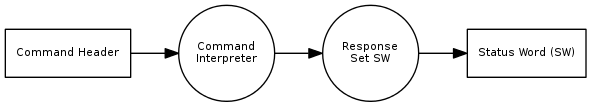
\includegraphics[width=0.75\textwidth]{image/command/dfd_cmdinterpreter.png}
\caption{DFD Command Interpreter}
\label{fig-dfd-cmdinterpreter}
\end{figure}

\begin{figure}[h]
\centering
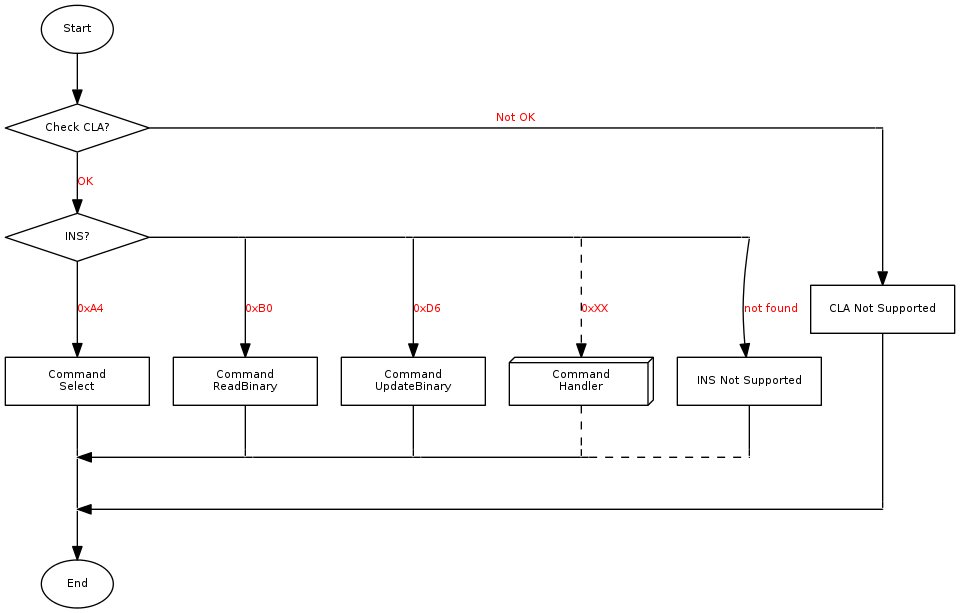
\includegraphics[width=0.9\textwidth, angle=90]{image/command/flow_cmdinterpreter.png}
\caption{Flowchart Command Interpreter}
\label{fig-flow-cmdinterpreter}
\end{figure}

\subsection {Pengujian}

\begin{table}[h]
  \centering
  \begin{tabular}{ | c || c | }
    \hline
    \bf{Input}  & \bf{Output} \\
    \hline
    \bf{Header} & \bf{Status Word}\\
    \hline
    [0x00,0x00,0x00.0x00,0x00] & = 6E00 (CLA Not Supported) \\
    \hline
    [0x80,0x00,0x00,0x00,0x00] & = 6D00 (INS Not Supported) \\
    \hline
    \multicolumn{2}{ |c| }{Include all test from Command Select} \\
    \hline
    \multicolumn{2}{ |c| }{Include all test from Read Binary} \\
    \hline
    \multicolumn{2}{ |c| }{Include all test from Update Binary} \\
    \hline
    \multicolumn{2}{ |c| }{Include all test from Create File} \\
    \hline
    \multicolumn{2}{ |c| }{Include all test from Delete File} \\
    \hline
    \multicolumn{2}{ |c| }{Include all test from Verify} \\
    \hline
    \multicolumn{2}{ |c| }{Include all test from Get Challenge} \\
    \hline
    \multicolumn{2}{ |c| }{Include all test from External Auth} \\
    \hline
    \multicolumn{2}{ |c| }{Include all test from Get Response} \\
    \hline
  \end{tabular}
  \caption{Test Vector Fungsi Command Interpreter}
  \label{tabel-test-cmdinterpreter}
\end{table}

Tabel \ref{tabel-test-cmdinterpreter} menampilkan Test Vector yang digunakan untuk menguji fungsi Command Interpreter.

\subsection {Implementasi}

Tabel \ref{tabel-cmdinterpreter} menampilkan purwarupa dari implementasi fungsi Command Interpreter. 

\begin{table}[h]
  \centering
  \begin{tabular}{m{2cm} p{8cm}}
    \hline\\
    {\bf Name} & Command\_Interpreter\\
    \hline\\
    {\bf Input} & -
    \\
    \hline\\
    {\bf Output} & -
    \\
    \hline
  \end{tabular}
  \caption{Prototype Fungsi Command Interpreter}
  \label{tabel-cmdinterpreter}
\end{table}

Listing \ref{list-cmdinterpreter} menampilkan kode program yang mengimplementasi fungsi Command Interpreter dan dapat ditemukan pada file $command.c$.

\begin{lstlisting}[caption={Implementasi Fungsi Command Interpreter},label={list-cmdinterpreter}]
void Command_Interpreter()
{
      if ( (header[0]&0xFC)==0x80 )
        {
          switch( header[1]&0xFE )
            {
            case ISO_SELECT:
              Command_Select();
              break;
            case ISO_READ_BINARY:
              Command_ReadBinary();
              break;
            case ISO_UPDATE_BINARY:
              Command_UpdateBinary();
              break;
            case ISO_CREATE_FILE:
              Command_CreateFile();
              break;
            case ISO_DELETE_FILE:
              Command_DeleteFile();
              break;
            case ISO_VERIFY:
              Command_Verify();
              break;
            case ISO_GET_CHALLENGE:
              Command_GetChallenge();
              break;
            case ISO_EXT_AUTH:
              Command_ExternalAuth();
              break;
            case ISO_GET_RESPONSE:
              Command_GetResponse();
              break;
            default:
              Response_SetSW( Response_INSNotSupported, 0 );
              break;
            }
        }
      else
        {
          Response_SetSW( Response_CLANotSupported, 0);
        }
}
\end{lstlisting}

\section{Command Handler - Select}
\label{sec_cmdselect}

Berfungsi sebagai command handler untuk instruksi Select. Gambar \ref{fig-dfd-cmdselect} menampilkan DFD dari fungsi Command Handler Select. Diagram alir fungsi kemudian ditampilkan pada Gambar \ref{fig-flow-cmdselect}. 

\begin{figure}[h]
\centering
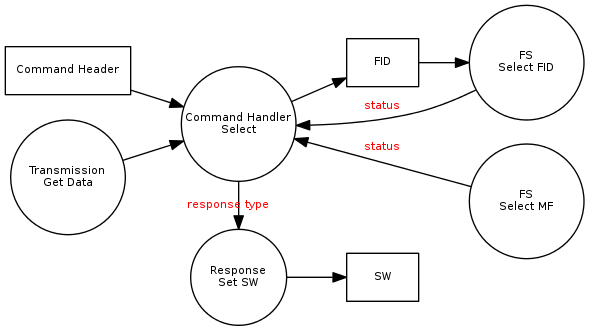
\includegraphics[width=0.75\textwidth]{image/command/dfd_cmdselect.png}
\caption{DFD Command Handler Select}
\label{fig-dfd-cmdselect}
\end{figure}

\begin{figure}
\centering
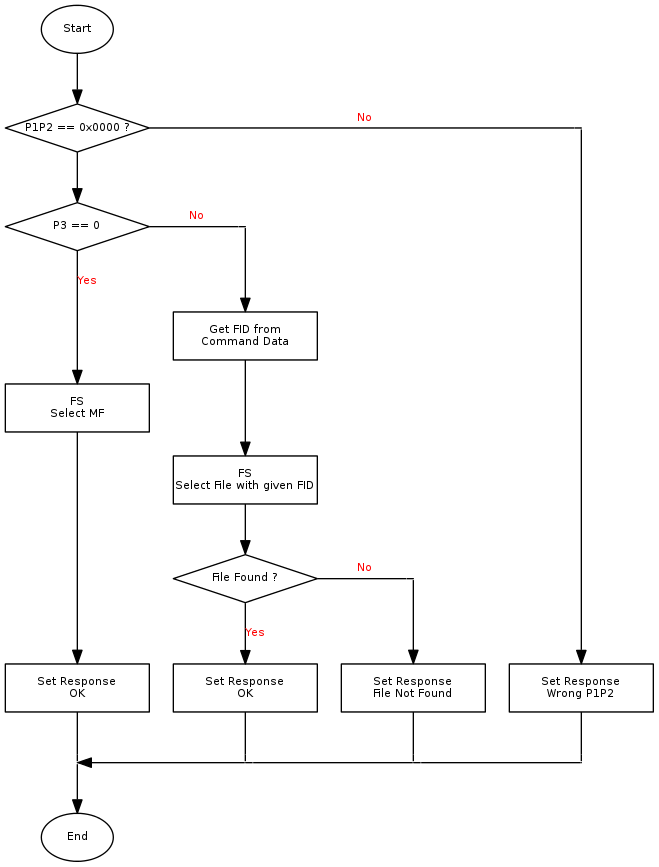
\includegraphics[width=0.75\textwidth]{image/command/flow_cmdselect.png}
\caption{Flowchart Command Handler Select}
\label{fig-flow-cmdselect}
\end{figure}

\subsection {Pengujian}

\begin{table}[h]
  \centering
  \begin{tabular}{ | c | c || c | }
    \hline
    \multicolumn{2}{ |c|| }{\bf{Input}}  & \bf{Output} \\
    \hline
    \bf{Header} & \bf{Data} & \bf{Status Word}\\
    \hline
    [0x80,0xA4,0x00.0x00,0x00] & - & = 9000 (OK) \\
    \hline
    [0x80,0xA4,0x00,0x00,0x02] & [3F,00] & = 9000 (OK) \\
    \hline
    [0x80,0xA4,0x00,0x00,0x02] & [FF,FF] & = 6A82 (File Not Found) \\
    \hline
    [0x80,0xA4,0xFF,0xFF,0x00] & - & = 6A00 (Wrong P1P2) \\
    \hline
  \end{tabular}
  \caption{Test Vector Fungsi Command Handler Select}
  \label{tabel-test-cmdselect}
\end{table}

Tabel \ref{tabel-test-cmdselect} menampilkan Test Vector yang digunakan untuk menguji fungsi Command Select.

\subsection {Implementasi}

\begin{table}[h]
  \centering
  \begin{tabular}{m{2cm} p{8cm}}
    \hline\\
    {\bf Name} & Command\_Select\\
    \hline\\
    {\bf Input} & -
    \\
    \hline\\
    {\bf Output} & -
    \\
    \hline
  \end{tabular}
  \caption{Prototype Fungsi Command Handler - Select}
  \label{tabel-cmdselect}
\end{table}

Tabel \ref{tabel-cmdselect} menampilkan purwarupa dari implementasi fungsi Command Select. 
Listing \ref{list-cmdselect} menampilkan potongan program yang mengimplementasi fungsi Command Handler Select

\begin{lstlisting}[caption={Listing Program Fungsi Command Handler Select}, label={list-cmdselect}]
void Command_Select()
{
  uint16_t fid, file;
  uint8_t data, temp;

  if((header[2] == 0x00) && (header[3]  == 0x00))
    {
      /* Select MF */
      if(header[4] == 0)
        {
          FSSelectMF();
          Response_SetSW(Response_OK, 0);
        }
      else
        {
          /* Get FID */
          Transmission_GetData(&temp,1);
          fid = (uint6_t) (temp) << 8;
          Transmission_GetData((&temp,1);
          fid |= (uint16_t) temp;

          /* Select with FID */
          switch( FS_SelectFID(fid) )
            {
            case FS_OK:
              Response_SetSW(Response_OK, 0);
              break;
            case FS_ERROR_NOT_FOUND:
              Response_SetSW( Response_WrongP1P2_FileNotFound, 0);
              break;              
            }
        }
    }
}
\end{lstlisting}


\section{Command Handler - Read Binary}
\label{sec_cmdread}

Berfungsi sebagai command handler untuk instruksi Read Binary. Gambar \ref{fig-dfd-cmdread} menampilkan DFD dari fungsi Command Handler Read Binary. Diagram alir fungsi kemudian ditampilkan pada Gambar \ref{fig-flow-cmdread}. 

\begin{figure}[h]
\centering
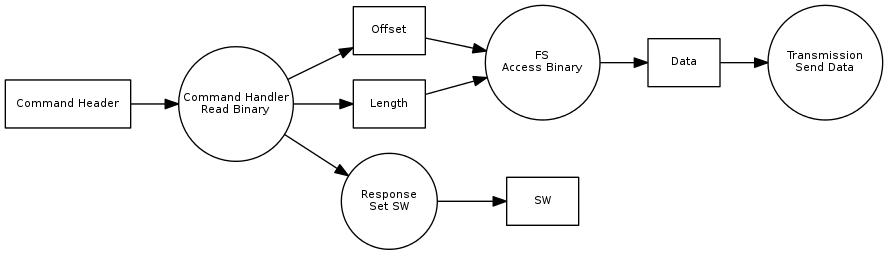
\includegraphics[width=0.75\textwidth]{image/command/dfd_cmdread.png}
\caption{DFD Command Read Binary}
\label{fig-dfd-cmdread}
\end{figure}

\begin{figure}
\centering
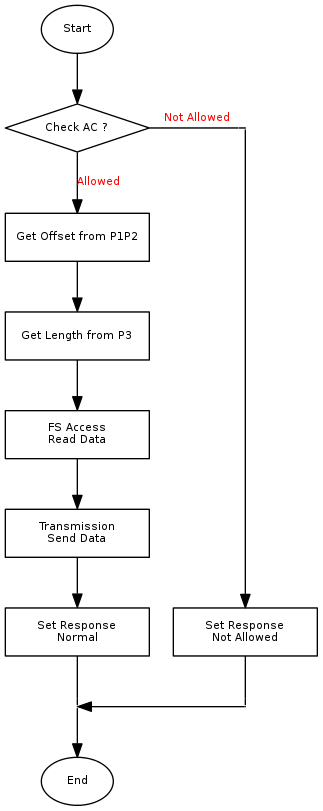
\includegraphics[width=0.5\textwidth]{image/command/flow_cmdread.png}
\caption{Flowchart Command Handler Read Binary}
\label{fig-flow-cmdread}
\end{figure}

\subsection {Pengujian}

\begin{table}[h]
  \centering
  \begin{tabular}{ | c || c | c | }
    \hline
    \bf{Input} & \multicolumn{2}{ c| }{\bf{Output}} \\
    \hline
    \bf{Header} & \bf{Data} & \bf{Status Word} \\
    \hline
    \multicolumn{3}{ |c| }{Create File with AC Read = 0} \\
    \multicolumn{3}{ |c| }{Select the last created file} \\
    \multicolumn{3}{ |c| }{Update File with data [1,2,3,4,5]} \\
    \hline
    {[0x80,0xB0,0x00.0x00,0x05]} & = [1,2,3,4,5] & = 6100 (Normal) \\
    \hline
    \multicolumn{3}{ |c| }{Create File with AC Read \ge 1} \\
    \multicolumn{3}{ |c| }{Select the last created file} \\
    \multicolumn{3}{ |c| }{Update File with data [1,2,3,4,5]} \\
    \hline
    {[0x80,0xB0,0x00,0x00,0x05]} & - & = 6982 (Not Allowed) \\
    \hline
  \end{tabular}
  \caption{Test Vector Fungsi Command Handler Read Binary}
  \label{tabel-test-cmdread}
\end{table}

Tabel \ref{tabel-test-cmdread} menampilkan Test Vector yang digunakan untuk menguji fungsi Command Read Binary.

\subsection {Implementasi}

Tabel \ref{tabel-cmdread} menampilkan purwarupa dari implementasi fungsi Command Read Binary.

\begin{table}[h]
  \centering
  \begin{tabular}{m{2cm} p{8cm}}
    \hline\\
    {\bf Name} & Command\_ReadBinary\\
    \hline\\
    {\bf Input} & -
    \\
    \hline\\
    {\bf Output} & -
    \\
    \hline
  \end{tabular}
  \caption{Prototype Fungsi Command Handler Read Binary}
  \label{tabel-cmdread}
\end{table}

Listing \ref{list-cmdread} menampilkan potongan program yang mengimplementasi fungsi Command Handler Read Binary

\begin{lstlisting}[caption={Kode Progrem Fungsi Command Handler Read Binary}, label={list-cmdread}]
void Command_ReadBinary()
{
  uint16_t offset, length;
  uint8_t data;

  HAL_IO_TxByte( header[1] );

  if( !(FS_CheckAC(FS_OP_READ) == FS_OK))
    {
      Response_SetSW( Response_CmdNotAllowed_SecurityStatus , 0);
      return;
    }

  offset = ((uint16_t)header[2] << 8) | header[3];

  uint8_t i;
  for( i=0; i<header[4]; i++ ) 
    {
      FSAccessBinary(FS_OP_READ,offset+i,1,&data);
      Transmission_SendData(&data,1);
    }

  Response_SetSW( Response_Normal, header[4]-i );
}
\end{lstlisting}

\section{Command Handler - Update}
\label{sec_cmdupdate}

Berfungsi sebagai command handler untuk instruksi Update Binary. Gambar \ref{fig-dfd-cmdupdate} menampilkan DFD dari fungsi Command Handler Update. Diagram alir fungsi kemudian ditampilkan pada Gambar \ref{fig-flow-cmdupdate}. 

\begin{figure}[h]
\centering
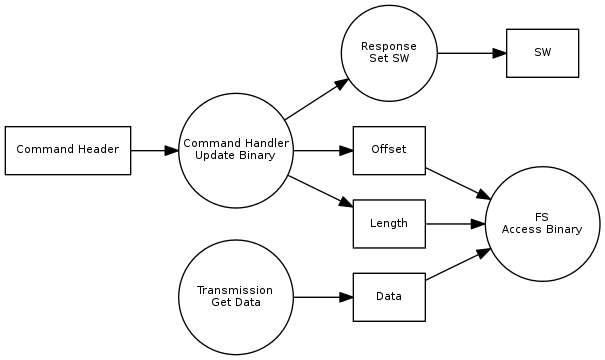
\includegraphics[width=0.75\textwidth]{image/command/dfd_cmdupdate.png}
\caption{DFD Command Update}
\label{fig-dfd-cmdupdate}
\end{figure}

\begin{figure}[h]
\centering
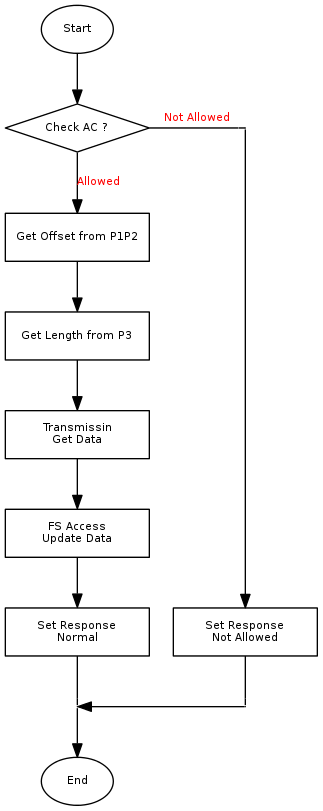
\includegraphics[height=0.6\textheight]{image/command/flow_cmdupdate.png}
\caption{Flowchart Command Handler Update}
\label{fig-flow-cmdupdate}
\end{figure}

\subsection {Pengujian}

\begin{table}[h]
  \centering
  \begin{tabular}{ | c || c | c | }
    \hline
    \multicolumn{2}{ |c| }{\bf{Input}} & {\bf{Output}} \\
    \hline
    \bf{Header} & \bf{Data} & \bf{Status Word} \\
    \hline
    \multicolumn{3}{ |c| }{Create File with AC Update = 0} \\
    \multicolumn{3}{ |c| }{Select the last created file} \\
    \hline
    {[0x80,0xB0,0x00.0x00,0x05]} & [1,2,3,4,5] & = 6100 (Normal) \\
    \hline
    \multicolumn{3}{ |c| }{Create File with AC Read \ge 1} \\
    \multicolumn{3}{ |c| }{Select the last created file} \\
    \hline
    {[0x80,0xD6,0x00,0x00,0x05]} & [1,2,3,4,5] & = 6982 (Not Allowed) \\
    \hline
  \end{tabular}
  \caption{Test Vector Fungsi Command Handler Update Binary}
  \label{tabel-test-cmdupdate}
\end{table}

Tabel \ref{tabel-test-cmdread} menampilkan Test Vector yang digunakan untuk menguji fungsi Command Read Binary.

\subsection {Implementasi}

Tabel \ref{tabel-cmdupdate} menampilkan purwarupa dari implementasi fungsi Command Update Binary.

\begin{table}[h]
  \centering
  \begin{tabular}{m{2cm} p{8cm}}
    \hline\\
    {\bf Name} & Command\_UpdateBinary\\
    \hline\\
    {\bf Input} & -
    \\
    \hline\\
    {\bf Output} & -
    \\
    \hline
  \end{tabular}
  \caption{Prototype Fungsi Command Handler Update}
  \label{tabel-cmdupdate}
\end{table}

Listing \ref{list-cmdupdate} menampilkan potongan program yang mengimplementasi fungsi Command Handler Update Binary.

\begin{lstlisting}[caption={Kode Program Fungsi Command Handler Update}, label={list-cmdupdate}]
void Command_UpdateBinary()
{
  uint16_t offset, length;
  uint8_t data;

  if( !(FS_CheckAC(FS_OP_UPDATE) == FS_OK))
    {
      Response_SetSW( Response_CmdNotAllowed_SecurityStatus , 0);
      return;
    }

  offset = ((uint16_t)(header[2]) << 8) | header[3];
  length = (uint16_t) header[4];

  uint8_t i;
  for( i=0; i<length; i++)
    {
      Transmission_GetData(&data,1);
      FSAccessBinary(FS_OP_UPDATE,offset+i,1,&data);
    }

  Response_SetSW( Response_Normal , 0);
}
\end{lstlisting}

\section{Command Handler - Create File}
\label{sec_cmdcreate}

Berfungsi sebagai command handler untuk instruksi Create File. Gambar \ref{fig-dfd-cmdcreate} menampilkan DFD dari fungsi Command Handler Create File. Diagram alir fungsi kemudian ditampilkan pada Gambar \ref{fig-flow-cmdcreate}. 

\begin{figure}[h]
\centering
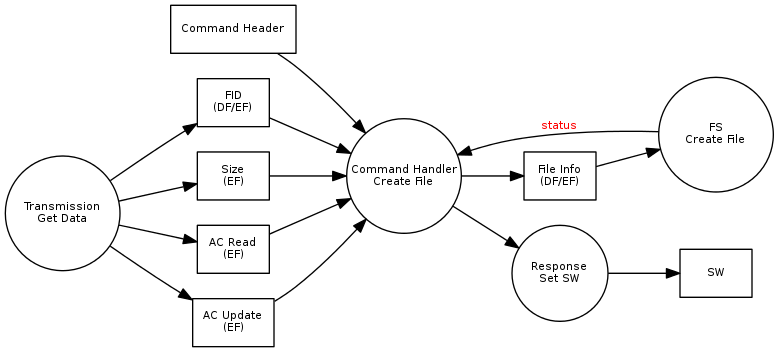
\includegraphics[width=0.75\textwidth]{image/command/dfd_cmdcreate.png}
\caption{DFD Command Create File}
\label{fig-dfd-cmdcreate}
\end{figure}

\begin{figure}[h]
\centering
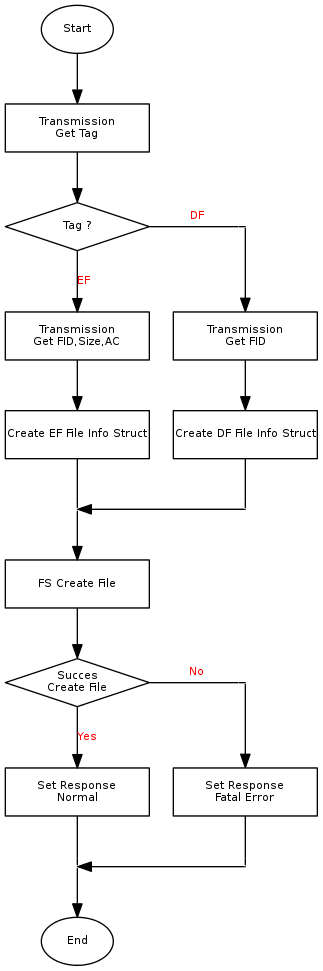
\includegraphics[height=0.6\textheight]{image/command/flow_cmdcreate.png}
\caption{Flowchart Command Handler Create File}
\label{fig-flow-cmdcreate}
\end{figure}

\subsection {Pengujian}

\begin{table}[h]
  \centering
  \begin{tabular}{ | c || c | c | }
    \hline
    \multicolumn{2}{ |c| }{\bf{Input}} & {\bf{Output}} \\
    \hline
    \bf{Header} & \bf{Data} & \bf{Status Word} \\
    \hline
    \multicolumn{3}{ |c| }{\emph{Create DF File}} \\
    \hline
    {[0x80,0xE0,0x00.0x00,0x03]} & [0x4f,0x12,0x34] & = 6100 (Normal) \\
    \hline
    \multicolumn{3}{ |c| }{\emph{Create DF with FID 3F00}} \\
    \hline
    {[0x80,0xE0,0x00.0x00,0x03]} & [0x4f,0x3f,0x00] & = 6F00 (Fatal Error) \\
    \hline
    \multicolumn{3}{ |c| }{\emph{Create EF with FID 5678}} \\
    \hline
    {[0x80,0xE0,0x00,0x00,0x07]} & [0x5f,0x56,0x78,0x00,0x05,0x00,0x00] & = 6100 (Normal) \\
    \hline
    \multicolumn{3}{ |c| }{\emph{Create EF with FID 5678 (same with the last created}} \\
    \hline
    {[0x80,0xE0,0x00,0x00,0x07]} & [0x5f,0x56,0x78,0x00,0x05,0x00,0x00] & = 6F00 (Fatal Error) \\
    \hline
  \end{tabular}
  \caption{Test Vector Fungsi Command Handler Update Binary}
  \label{tabel-test-cmdupdate}
\end{table}

Tabel \ref{tabel-test-cmdread} menampilkan Test Vector yang digunakan untuk menguji fungsi Command Read Binary.

\subsection {Implementasi}

Tabel \ref{tabel-cmdcreate} menampilkan purwarupa dari implementasi fungsi Command Create File.

\begin{table}[h]
  \centering
  \begin{tabular}{m{2cm} p{8cm}}
    \hline\\
    {\bf Name} & Command\_CreateFile\\
    \hline\\
    {\bf Input} & -
    \\
    \hline\\
    {\bf Output} & -
    \\
    \hline
  \end{tabular}
  \caption{Prototype Fungsi Command Handler Create File}
  \label{tabel-cmdcreate}
\end{table}

Listing \ref{list-cmdcreate} menampilkan potongan program yang mengimplementasi fungsi Command Handler Create File

\begin{lstlisting}[caption={Listing Program Fungsi Command Handler Create File}, label{list-cmdcreate}]
void Command_CreateFile()
{
  uint8_t tag;
  uint16_t size, fid;
  uint8_t acread, acupdate;
  uint8_t result;
  uint8_t temp;

  /* Get Tag */
  Transmissin_GetData(&tag,1)

  switch( tag )
    {
    case FS_TAG_DF:
      /* Get FID */
      Transmission_GetData(&temp,1);
      fid = (uint6_t) (temp) << 8;
      Transmission_GetData((&temp,1);
      fid |= (uint16_t) temp;

      struct DF_st df;
      df.FID = fid;

      result = FSCreateFile(tag,&df);
      break;
    case FS_TAG_EF:
      /* Get FID */
      Transmission_GetData(&temp,1);
      fid = (uint6_t) (temp) << 8;
      Transmission_GetData((&temp,1);
      fid |= (uint16_t) temp;

      /* Get Size */
      Transmission_GetData(&temp,1);
      size = (uint6_t) (temp) << 8;
      Transmission_GetData((&temp,1);
      size |= (uint16_t) temp;

      /* Get AC for Read */
      Transmission_GetData(&acread,1);

      /* Get AC for Update */
      Transmission_GetData(&acupdate,1);

      struct EF_st ef;

      ef.FID = fid;
      ef.structure = FS_EF_STRUCTURE_TRANSPARENT;
      ef.type = FS_EF_TYPE_WORKING;
      ef.ACRead = acread; //(ac && 0xf0) >> 4;
      ef.ACUpdate = acupdate; //ac && 0x0f;
      ef.size = size;

      result = FSCreateFile(tag,&ef);

      break;
    }

  switch ( result )
    {
    case FS_OK:
      Response_SetSW( Response_Normal , 0);
      break;
    default:
      Response_SetSW( Response_FatalError , 0);
      break;
    }
}
\end{lstlisting}

\section{Command Handler - Delete File}
\label{sec_cmddelete}

Berfungsi sebagai command handler untuk instruksi Delete File. Gambar \ref{fig-dfd-cmddelete} menampilkan DFD dari fungsi Command Handler Delete File. Diagram alir fungsi kemudian ditampilkan pada Gambar \ref{fig-flow-cmddelete}. 

\begin{figure}[h]
\centering
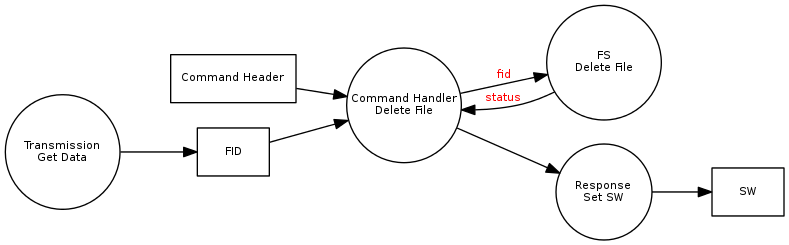
\includegraphics[width=0.75\textwidth]{image/command/dfd_cmddelete.png}
\caption{DFD Command Delete File}
\label{fig-dfd-cmddelete}
\end{figure}

\begin{figure}[h]
\centering
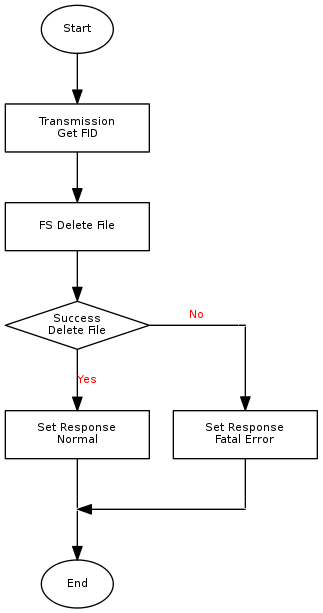
\includegraphics[height=0.6\textheight]{image/command/flow_cmddelete.png}
\caption{Flowchart Command Handler Delete File}
\label{fig-flow-cmddelete}
\end{figure}

\subsection {Pengujian}

\begin{table}[h]
  \centering
  \begin{tabular}{ | c || c | c | }
    \hline
    \multicolumn{2}{ |c| }{\bf{Input}} & {\bf{Output}} \\
    \hline
    \bf{Header} & \bf{Data} & \bf{Status Word} \\
    \hline
    \multicolumn{3}{ |c| }{\bf{Description :}} \\
    \multicolumn{3}{ |c| }{\emph{Delete Existence File}} \\
    \multicolumn{3}{ |c| }{\bf{Setup :}} \\
    \multicolumn{3}{ |c| }{\emph{Create File with FID 1234}} \\
    \hline
    {[0x80,0xE4,0x00.0x00,0x02]} & [0x12,0x34] & = 6100 (Normal) \\
    \hline
    \multicolumn{3}{ |c| }{\bf{Description :}} \\
    \multicolumn{3}{ |c| }{\emph{Delete Non-existence File}} \\
    \hline
    {[0x80,0xE4,0x00.0x00,0x03]} & [0x56,0x78] & = 6F00 (Fatal Error) \\
    \hline
  \end{tabular}
  \caption{Test Vector Fungsi Command Handler Delete File}
  \label{tabel-test-cmddelete}
\end{table}

Tabel \ref{tabel-test-cmddelete} menampilkan Test Vector yang digunakan untuk menguji fungsi Command Handler Delete File.


\subsection {Implementasi}

Tabel \ref{tabel-cmddelete} menampilkan purwarupa dari implementasi fungsi Command Delete File.

\begin{table}[h]
  \centering
  \begin{tabular}{p{2cm} p{8cm}}
    \hline\\
    {\bf Name} & Command\_DeleteFile\\
    \hline\\
    {\bf Input} & -
    \\
    \hline\\
    {\bf Output} & -
    \\
    \hline
  \end{tabular}
  \caption{Prototype Fungsi Command Handler Delete File}
  \label{tabel-cmddelete}
\end{table}

Listing \ref{list-cmddelete} menampilkan kode program yang mengimplementasi fungsi Command Handler Delete File

\begin{lstlisting}[caption={Kode Program Fungsi Command Handler Delete File}, label={list-cmddelete}]
void Command_DeleteFile()
{
  uint16_t fid;
  uint8_t temp;

  /* Get FID */
  Transmission_GetData(&temp,1);
  fid = (uint6_t) (temp) << 8;
  Transmission_GetData((&temp,1);
  fid |= (uint16_t) temp;

  switch ( FSDeleteFile(fid) )
    {
    case FS_OK:
      Response_SetSW( Response_Normal , 0);
      break;
    default:
      Response_SetSW( Response_FatalError , 0);
      break;
    }
}
\end{lstlisting}


\section{Command Handler - Verify PIN}
\label{sec_cmdverify}

\begin{figure}[h]
\centering
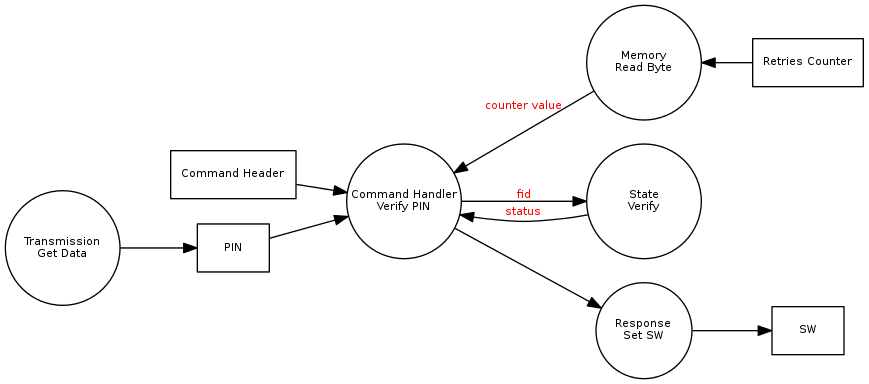
\includegraphics[width=0.75\textwidth]{image/command/dfd_cmdverify.png}
\caption{DFD Command Handler Verify}
\label{fig-dfd-cmdverify}
\end{figure}

Berfungsi sebagai command handler untuk instruksi Verify. Gambar \ref{fig-dfd-cmdverify} menampilkan DFD dari fungsi Command Handler Verify. Diagram alir fungsi kemudian ditampilkan pada Gambar \ref{fig-flow-cmdverify}. 

\begin{figure}[h]
\centering
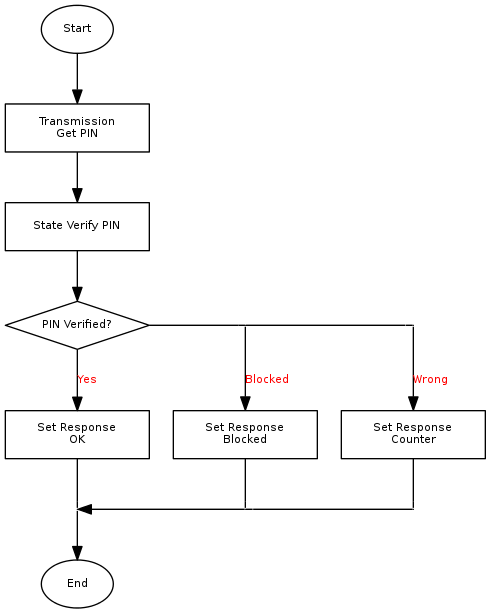
\includegraphics[height=0.4\textheight]{image/command/flow_cmdverify.png}
\caption{Flowchart Command Handler Verify}
\label{fig-flow-cmdverify}
\end{figure}

\subsection {Pengujian}

\begin{table}[h]
  \centering
  \begin{tabular}{ | c || c | c | }
    \hline
    \multicolumn{2}{ |c| }{\bf{Input}} & {\bf{Output}} \\
    \hline
    \bf{Header} & \bf{Data} & \bf{Status Word} \\
    \hline
    \multicolumn{3}{ |c| }{\bf{Description :}} \\
    \multicolumn{3}{ |c| }{\emph{Verify with Correct PIN}} \\
    \multicolumn{3}{ |c| }{\bf{Setup :}} \\
    \multicolumn{3}{ |c| }{\emph{Correct PIN = 1234}} \\
    \hline
    {[0x80,0x20,0x00.0x00,0x04]} & [1,2,3,4] & = 9000 (OK) \\
    \hline
    \multicolumn{3}{ |c| }{\bf{Description :}} \\
    \multicolumn{3}{ |c| }{\emph{Verify with Incorrect PIN until blocked}} \\
    \multicolumn{3}{ |c| }{\bf{Setup :}} \\
    \multicolumn{3}{ |c| }{\emph{Correct PIN = 1234}} \\
    \multicolumn{3}{ |c| }{\emph{Max. Try = 3}} \\
    \hline
    {[0x80,0x20,0x00.0x00,0x04]} & [4,3,2,1] & = 63C1 (Counter) \\
    {[0x80,0x20,0x00.0x00,0x04]} & [4,3,2,1] & = 63C2 (Counter) \\
    {[0x80,0x20,0x00.0x00,0x04]} & [4,3,2,1] & = 63C3 (Counter) \\
    {[0x80,0x20,0x00.0x00,0x04]} & [4,3,2,1] & = 6383 (Auth Blocked) \\
    \hline
  \end{tabular}
  \caption{Test Vector Fungsi Command Handler Verify}
  \label{tabel-test-cmdverify}
\end{table}

Tabel \ref{tabel-test-cmdverify} menampilkan Test Vector yang digunakan untuk menguji fungsi Command Handler Verify.


\subsection {Implementasi}

Tabel \ref{tabel-cmdverify} menampilkan purwarupa dari implementasi fungsi Command Handler Verify.

\begin{table}[h]
  \centering
  \begin{tabular}{p{2cm} p{8cm}}
    \hline\\
    {\bf Name} & Command\_Verify\\
    \hline\\
    {\bf Input} & -
    \\
    \hline\\
    {\bf Output} & -
    \\
    \hline
  \end{tabular}
  \caption{Prototype Fungsi Command Handler Verify}
  \label{tabel-cmdverify}
\end{table}

Listing \ref{list-cmdverify} menampilkan potongan program yang mengimplementasi fungsi Command Handler Verify.

\begin{lstlisting}[caption={Listing Program Fungsi Command Handler Verify}, label={list-cmdverify}]
void Command_Verify()
{
  uint8_t pin[PIN_LEN];

  if( header[4] != PIN_LEN )
    {
      Response_SetSW( Response_WrongLength , 0);
      return;
    }

  /* Get PIN */
  Transmission_GetData(pin, PIN_LEN);

  uint8_t retries;
  switch( State_Verify(pin) )
    {
    case STATE_OK:
      Response_SetSW( Response_OK , 0);
      break;
    case STATE_BLOCKED:
      Response_SetSW( Response_CmdNotAllowed_AuthBlocked , 0);
      break;
    case STATE_WRONG:
      retries = Memory_ReadByte(PIN_RETRIES_ADDR);
      Response_SetSW( Response_Warning_Counter | (retries & 0x0f) , 0);
    }
}
\end{lstlisting}

\section{Command Handler - Get Challenge}
\label{sec_cmdgetchallenge}

Berfungsi sebagai command handler untuk instruksi Get Challenge. Gambar \ref{fig-dfd-cmdgetchallenge} menampilkan DFD dari fungsi Command Handler Get Challenge. Diagram alir fungsi kemudian ditampilkan pada Gambar \ref{fig-flow-cmdgetchallenge}. 

\begin{figure}[h]
\centering
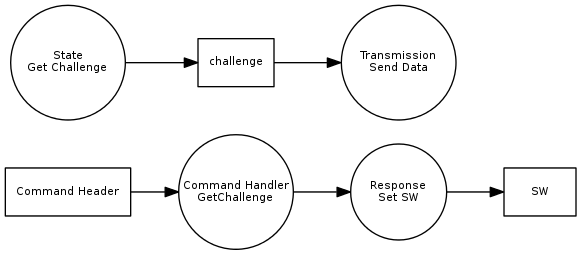
\includegraphics[width=0.6\textwidth]{image/command/dfd_cmdgetchallenge.png}
\caption{DFD Command Handler Get Challenge}
\label{fig-dfd-cmdgetchallenge}
\end{figure}

\begin{figure}[h]
\centering
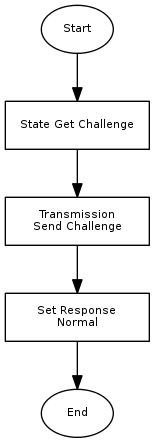
\includegraphics[height=0.5\textheight]{image/command/flow_cmdgetchallenge.png}
\caption{Flowchart Command Handler Get Challenge}
\label{fig-flow-cmdgetchallenge}
\end{figure}

\subsection {Pengujian}

\begin{table}[h]
  \centering
  \begin{tabular}{ | c || c | c | }
    \hline
    {\bf{Input}} & \multicolumn{2}{ |c| }{\bf{Output}} \\
    \hline
    \bf{Header} & \bf{Data} & \bf{Status Word} \\
    \hline
    {[0x80,0x84,0x00.0x00,0x08]} & x,x,x,x,x & = 6100 (Normal) \\
    \hline
  \end{tabular}
  \caption{Test Vector Fungsi Command Handler Get Challenge}
  \label{tabel-test-cmdgetchallenge}
\end{table}

Tabel \ref{tabel-test-cmdgetchallenge} menampilkan Test Vector yang digunakan untuk menguji fungsi Command Handler Get Challenge.

\subsection {Implementasi}

Tabel \ref{tabel-cmdgetchallenge} menampilkan purwarupa dari implementasi fungsi Command Handler Get Challenge.

\begin{table}[h]
  \centering
  \begin{tabular}{p{2cm} p{8cm}}
    \hline\\
    {\bf Name} & Command\_GetChallenge\\
    \hline\\
    {\bf Input} & -
    \\
    \hline\\
    {\bf Output} & -
    \\
    \hline
  \end{tabular}
  \caption{Prototype Fungsi Command Handler Get Challenge}
  \label{tabel-cmdgetchallenge}
\end{table}

Listing \ref{list-cmdgetchallenge} menampilkan potongan program yang mengimplementasi fungsi Command Handler Get Challenge.

\begin{lstlisting}[caption={Listing Program Fungsi Command Handler Get Challenge}, label={list-cmdgetchallenge}]
void Command_GetChallenge()
{
	uint8_t buf[CRYPT_BLOCK_LEN];

	if( !(header[4] == CRYPT_BLOCK_LEN ) )
          {
            Response_SetSW( Response_WrongLength , 0);
            return;
          }

	/* ACK */
        HAL_IO_TxByte( header[1] );

	State_GetChallenge( buf );

        Transmission_SendData(buf, CRYPT_BLOCK_LEN);

        Response_SetSW( Response_Normal , 0);
}
\end{lstlisting}


\section{Command Handler - External Authentication}
\label{sec_cmdextauth}

Berfungsi sebagai command handler untuk instruksi External Authentication. Gambar \ref{fig-dfd-cmdextauth} menampilkan DFD dari fungsi Command Handler External Auth. Diagram alir fungsi kemudian ditampilkan pada Gambar \ref{fig-flow-cmdextauth}. 

\begin{figure}[h]
\centering
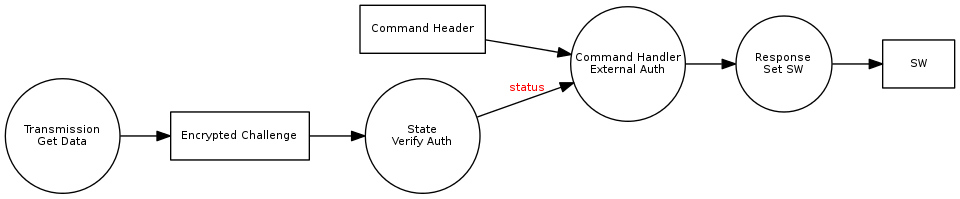
\includegraphics[width=0.75\textwidth]{image/command/dfd_cmdextauth.png}
\caption{DFD Command External Auth}
\label{fig-dfd-cmdextauth}
\end{figure}

\begin{figure}[h]
\centering
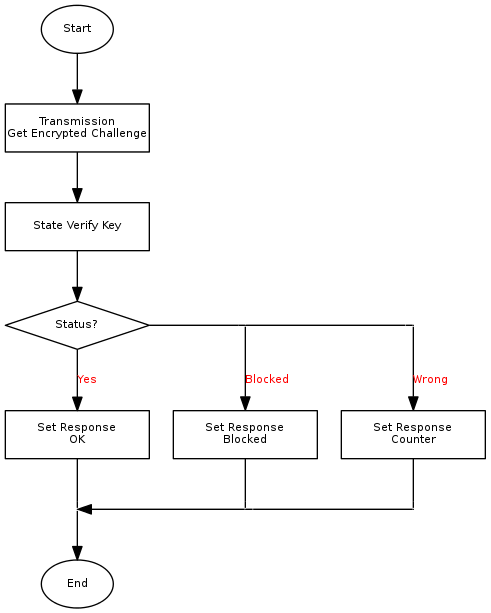
\includegraphics[height=0.5\textheight]{image/command/flow_cmdextauth.png}
\caption{Flowchart Command Handler External Auth}
\label{fig-flow-cmdextauth}
\end{figure}

\subsection {Pengujian}

\begin{table}[h]
  \centering
  \begin{tabular}{ | c || c | c | }
    \hline
    \multicolumn{2}{ |c| }{\bf{Input}} & {\bf{Output}} \\
    \hline
    \bf{Header} & \bf{Data} & \bf{Status Word} \\
    \hline
    \multicolumn{3}{ |c| }{\bf{Description :}} \\
    \multicolumn{3}{ |c| }{\emph{Verify with Correct Encrypted Challenge}} \\
    \multicolumn{3}{ |c| }{\bf{Setup :}} \\
    \multicolumn{3}{ |c| }{\emph{create challenge}} \\
    \multicolumn{3}{ |c| }{\emph{encrypted challenge = xxxxxxxx}} \\
    \hline
    {[0x80,0x82,0x00.0x00,0x08]} & xxxxxxxx & = 9000 (OK) \\
    \hline
    \multicolumn{3}{ |c| }{\bf{Description :}} \\
    \multicolumn{3}{ |c| }{\emph{Verify with Incorrect Encrypted Challenge}} \\
    \multicolumn{3}{ |c| }{\bf{Setup :}} \\
    \multicolumn{3}{ |c| }{\emph{encrypted challenge = xxxxxxxx}} \\
    \hline
    {[0x80,0x82,0x00.0x00,0x04]} & ~xxxxxxxx & = 63C1 (Counter) \\
    {[0x80,0x82,0x00.0x00,0x04]} & ~xxxxxxxx & = 63C2 (Counter) \\
    {[0x80,0x82,0x00.0x00,0x04]} & ~xxxxxxxx & = 63C3 (Counter) \\
    {[0x80,0x82,0x00.0x00,0x04]} & ~xxxxxxxx & = 6383 (Auth Blocked) \\
    \hline
  \end{tabular}
  \caption{Test Vector Fungsi Command Handler External Authentication}
  \label{tabel-test-cmdextauth}
\end{table}

Tabel \ref{tabel-test-cmdextauth} menampilkan Test Vector yang digunakan untuk menguji fungsi Command Handler Verify.

\subsection {Implementasi}

Tabel \ref{tabel-cmdextauth} menampilkan purwarupa dari implementasi fungsi Command Handler External Authentication.

\begin{table}[h]
  \centering
  \begin{tabular}{p{2cm} p{8cm}}
    \hline\\
    {\bf Name} & Command\_ExternalAuth\\
    \hline\\
    {\bf Input} & -
    \\
    \hline\\
    {\bf Output} & -
    \\
    \hline
  \end{tabular}
  \caption{Prototype Fungsi Command Handler External Authentication}
  \label{tabel-cmdextauth}
\end{table}

Listing \ref{list-cmdextauth} menampilkan potongan program yang mengimplementasi fungsi Command Handler External Authentication.

\begin{lstlisting}[caption={Listing Program Fungsi Command Handler External Auth}, label={list-cmdextauth}]
void Command_ExternalAuth()
{
  uint8_t encrypted[CRYPT_BLOCK_LEN];
  uint8_t i;

  if( !(header[4] == CRYPT_BLOCK_LEN) )
    {
      Response_SetSW( Response_WrongLength , 0);
      return;
    }

  Transmission_GetData(encrypted, CRYPT_BLOCK_LEN];

  uint8_t retries;
  switch( State_VerifyAuth( &encrypted ) )
    {
    case STATE_OK:
      Response_SetSW( Response_OK , 0);
      break;
    case STATE_BLOCKED:
      Response_SetSW( Response_CmdNotAllowed_AuthBlocked , 0);
      break;
    case STATE_WRONG:
      retries = Memory_ReadByte(EXT_AUTH_RETRIES_ADDR);
      Response_SetSW( Response_Warning_Counter | (retries & 0x0f) , 0);
    }

}
\end{lstlisting}

\section{Command Handler - Get Response}
\label{sec_cmdgetresponse}

Berfungsi sebagai command handler untuk instruksi Get Response. Gambar \ref{fig-dfd-cmdgetresponse} menampilkan DFD dari fungsi Command Handler Get Response. Diagram alir fungsi kemudian ditampilkan pada Gambar \ref{fig-flow-cmdgetresponse}. 

\begin{figure}[h]
\centering
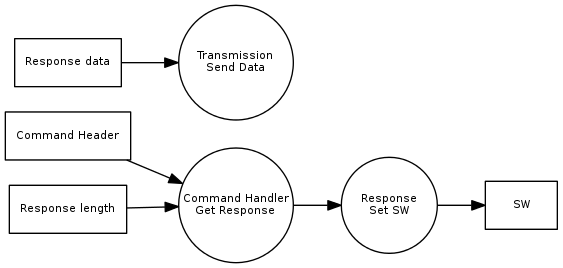
\includegraphics[width=0.74\textwidth]{image/command/dfd_cmdgetresponse.png}
\caption{DFD Command Get Response}
\label{fig-dfd-cmdgetresponse}
\end{figure}

\begin{figure}[h]
\centering
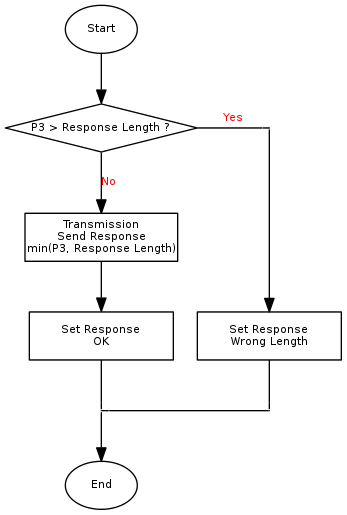
\includegraphics[height=0.5\textheight]{image/command/flow_cmdgetresponse.png}
\caption{Flowchart Command Handler Get Response}
\label{fig-flow-cmdgetresponse}
\end{figure}

\subsection {Pengujian}

\begin{table}[h]
  \centering
  \begin{tabular}{ | c || c | c | }
    \hline
    {\bf{Input}} & \multicolumn{2}{ |c| }{\bf{Output}} \\
    \hline
    \bf{Header} & \bf{Data} & \bf{Status Word} \\
    \hline
    \multicolumn{3}{ |c| }{\bf{Setup :}} \\
    \multicolumn{3}{ |c| }{\emph{response = [1,2,3,4,5]}} \\
    \multicolumn{3}{ |c| }{\emph{resplen = 5}} \\
    \hline
    {[0x80,0xC0,0x00.0x00,0x05]} & = [1,2,3,4,5] & = 6100 (Normal) \\
    {[0x80,0xC0,0x00.0x00,0x03]} & = [1,2,3] & = 6100 (Normal) \\
    {[0x80,0xC0,0x00.0x00,0x08]} & - & = 6700 (Wrong Length) \\
    \hline
  \end{tabular}
  \caption{Test Vector Fungsi Command Handler Get Response}
  \label{tabel-test-cmdgetresponse}
\end{table}

Tabel \ref{tabel-test-cmdgetresponse} menampilkan Test Vector yang digunakan untuk menguji fungsi Command Handler Get Response.

\subsection {Implementasi}

Tabel \ref{tabel-cmdgetresponse} menampilkan purwarupa dari implementasi fungsi Command Handler Get Response.

\begin{table}[h]
  \centering
  \begin{tabular}{p{2cm} p{8cm}}
    \hline\\
    {\bf Name} & Command\_GetResponse\\
    \hline\\
    {\bf Input} & Command Header
    \\
    \hline\\
    {\bf Output} & 
    \\
    \hline
  \end{tabular}
  \caption{Prototype Fungsi Command Handler Get Response}
  \label{tabel-cmdgetresponse}
\end{table}

Listing \ref{list-cmdgetresponse} menampilkan potongan program yang mengimplementasi fungsi Command Handler Get Response

\begin{lstlisting}[caption={Listing Program Fungsi Command Handler Get Response}, label={list_cmdgetresponse}]
void Command_GetResponse()
{
  if( resplen==0 ) {
    Response_SetSW( Response_CmdNotAllowed_ConditionNotSatisfied , 0);
    return;
  }

  if( (header[4]>resplen) || (!header[4]) ) {
    Response_SetSW( Response_WrongLength , 0);
    return;
  }
  resplen=header[4];

  /* ACK */
  HAL_IO_TxByte( header[1] );

  Transmission_SendData(response,resplen);

  Response_SetSW( Response_Normal , 0);
}
\end{lstlisting}

